\documentclass[10pt,winfonts,fancyhdr,hyperref,UTF8]{ctexrep}
\usepackage{indentfirst} 
\usepackage{fontspec}
\usepackage{titlesec}
\usepackage{xeCJK}
\usepackage{graphicx}
\usepackage{ifthen}
\usepackage{color,fancyvrb}
\usepackage{listings}
\usepackage{syntonly}
\usepackage{makeidx}
\usepackage[hidelinks, colorlinks=true]{hyperref}
\usepackage{algorithm}
\usepackage{algpseudocode}
\usepackage{amssymb}
\usepackage{multirow}
\usepackage{ulem}
\usepackage{diagbox}
\makeatletter
%LeetCode Setting
\usepackage[centering,paperwidth=180mm,paperheight=230mm,%
body={390pt,530pt},marginparsep=10pt,marginpar=50pt]{geometry}
\usepackage{color}
\usepackage{enumitem}
\usepackage{fancyvrb}
\usepackage[bottom,perpage,symbol*]{footmisc}
\usepackage{graphicx}
\usepackage[hidelinks]{hyperref}
\usepackage{makeidx}
\usepackage[toc]{multitoc}
\usepackage{pifont}
\usepackage{underscore}
\usepackage{amsmath}

\DefineFNsymbols*{chinese}{{\ding{172}}{\ding{173}}{\ding{174}}{\ding{175}}%
{\ding{176}}{\ding{177}}{\ding{178}}{\ding{179}}{\ding{180}}{\ding{181}}}
\setfnsymbol{chinese}

\hypersetup{bookmarksnumbered=true,bookmarksdepth=2}

\CTEXsetup[number={\thechapter}]{chapter}
\CTEXsetup[format+={\raggedleft}]{chapter}
\CTEXsetup[beforeskip={10pt}]{chapter}
\CTEXsetup[afterskip={30pt}]{chapter}
\def\CTEX@chapter@aftername{\par} % \CTEXsetup[aftername={\par}]{chapter}
\CTEXsetup[format+={\raggedright}]{section}
\CTEXsetup[beforeskip={-3.0ex plus -1ex minus -.2ex}]{section}
\CTEXsetup[afterskip={2.3ex plus .2ex minus 0.2ex}]{section}

\renewcommand \thefigure{\thechapter-\arabic{figure}}
\renewcommand \thetable{\thechapter-\arabic{table}}

\newcommand\figcaption[1]{\def\@captype{figure}\caption{#1}}
\newcommand\tabcaption[1]{\def\@captype{table}\caption{#1}}

\long\def\@caption#1[#2]#3{%
  \addcontentsline{\csname ext@#1\endcsname}{#1}%
    {\protect\numberline{\csname fnum@#1\endcsname}{ \ignorespaces #2}}% change "the" to "fnum@"
    \normalsize
    \@makecaption{\csname fnum@#1\endcsname}{\ignorespaces #3}}

\long\def\@makecaption#1#2{%
  \vskip\abovecaptionskip
  \sbox\@tempboxa{#1\quad#2}%
  \ifdim \wd\@tempboxa >\hsize
    #1\quad#2\par
  \else
    \global \@minipagefalse
    \hb@xt@\hsize{\hfil\box\@tempboxa\hfil}%
  \fi
  \vskip\belowcaptionskip}

\setlength\abovecaptionskip{0pt}
  
\setmainfont{Times New Roman}
%\setmainfont{Linux Libertine}
%\setmainfont{TeX Gyre Pagella}
\newfontfamily\urlfont{Times New Roman}
%\setmonofont[AutoFakeBold=1.6,AutoFakeSlant=0.17,Mapping=tex-text-tt]{Inconsolata}
\setCJKfamilyfont{zhyou}{YouYuan}

\newcommand{\fn}[1]{\texttt{#1}}
\newcommand{\sfn}[1]{\texttt{\small #1}}
\newcommand{\kw}[1]{\textsf{#1}}
\newcommand{\myurl}[1]{{\urlfont #1}}
\newcommand{\mpar}[1]{\marginpar[\hfill\kaishu #1]{\kaishu #1}}
\newcommand{\mn}[1]{\texttt{\bs #1}}
\renewcommand{\today}{\the\year-\the\month-\the\day}
\newcommand\bs{\textbackslash}
\newcommand{\code}[1]{\small{\fontspec{Latin Modern Mono} #1}}

\newcommand\begindot{\begin{itemize}
[itemsep=2pt plus 2pt minus 2pt,%
topsep=3pt plus 2pt minus 2pt,%
parsep=0pt plus 2pt minus 2pt]}
\newcommand\myenddot{\end{itemize}}

\newcommand\beginnum{\begin{enumerate}
[itemsep=2pt plus 2pt minus 2pt,%
topsep=3pt plus 2pt minus 2pt,%
parsep=0pt plus 2pt minus 2pt]}
\newcommand\myendnum{\end{enumerate}}

\DefineVerbatimEnvironment%
  {Code}{Verbatim}
  {fontsize=\small,baselinestretch=0.9,xleftmargin=3mm}

\raggedbottom
%\setlength{\parskip}{1ex plus .5ex minus .5ex}

\def\FV@SetLineWidth{%
  \if@FV@ResetMargins\else
    \advance\leftmargin\@totalleftmargin
  \fi
  \advance\leftmargin\FV@XLeftMargin\relax
  \advance\rightmargin\FV@XRightMargin\relax
  \linewidth\hsize
  %\advance\linewidth-\leftmargin
  %\advance\linewidth-\rightmargin
  \hfuzz\FancyVerbHFuzz\relax}


\def\FV@SingleFrameLine#1{%
%% DG/SR modification end
  \hbox to\z@{%
    %\kern\leftmargin
%% DG/SR modification begin - Jun. 22, 1998
    \ifnum#1=\z@
      \let\FV@Label\FV@LabelBegin
    \else
      \let\FV@Label\FV@LabelEnd
    \fi
    \ifx\FV@Label\relax
%% DG/SR modification end
      \FancyVerbRuleColor{\vrule \@width\linewidth \@height\FV@FrameRule}%
%% DG/SR modification begin - Jun. 22, 1998
    \else
      \ifnum#1=\z@
        \setbox\z@\hbox{\strut\enspace\urlfont\FV@LabelBegin\strut}%
      \else
        \setbox\z@\hbox{\strut\enspace\urlfont\FV@LabelEnd\strut}%
      \fi
      \@tempdimb=\dp\z@
      \advance\@tempdimb -.5\ht\z@
      \@tempdimc=\linewidth
      \advance\@tempdimc -\wd\z@
      %\divide\@tempdimc\tw@
      \ifnum#1=\z@              % Top line
        \ifx\FV@LabelPositionTopLine\relax
          \FancyVerbRuleColor{\vrule \@width\linewidth \@height\FV@FrameRule}%
        \else
          \FV@FrameLineWithLabel
        \fi
      \else                     % Bottom line
        \ifx\FV@LabelPositionBottomLine\relax
          \FancyVerbRuleColor{\vrule \@width\linewidth \@height\FV@FrameRule}%
        \else
          \FV@FrameLineWithLabel
        \fi
      \fi
    \fi
%% DG/SR modification end
    \hss}}


%% DG/SR modification begin - May. 19, 1998
\def\FV@FrameLineWithLabel{%
  \ht\z@\@tempdimb\dp\z@\@tempdimb%
  \FancyVerbRuleColor{%
    \raise 0.5ex\hbox{\vrule \@width\@tempdimc \@height\FV@FrameRule}%
    \raise\@tempdimb\box\z@}}
%% DG/SR modification end


\def\FV@EndListFrame@Lines{%
  \begingroup
    %\vskip 0.5ex
    \baselineskip\z@skip
    \kern\FV@FrameSep\relax
%% DG/SR modification begin - May. 19, 1998
%%    \FV@SingleFrameLine
    \FV@SingleFrameLine{\@ne}%
%% DG/SR modification end
  \endgroup}

\newskip\mytopsep
\setlength{\mytopsep}{4pt plus 2pt minus 3pt}

\def\FV@ListVSpace{%
  \@topsepadd\mytopsep
  \if@noparlist\advance\@topsepadd\partopsep\fi
  \if@inlabel
    \vskip\parskip
  \else
    \if@nobreak
      \vskip\parskip
      \clubpenalty\@M
    \else
      \addpenalty\@beginparpenalty
      \@topsep\@topsepadd
      \advance\@topsep\parskip
      \addvspace\@topsep
    \fi
  \fi
  %\showthe \@topsepadd
  %\showthe \topsep
  %\showthe \partopsep
  %\showthe \parskip
  \global\@nobreakfalse
  \global\@inlabelfalse
  \global\@minipagefalse
  \global\@newlistfalse}

\def\FV@EndList{%
  \FV@ListProcessLastLine
  \FV@EndListFrame
  %\showthe \@topsepadd
  \@endparenv
  \endgroup
  \@endpetrue}

\def\theFancyVerbLine{\sffamily\scriptsize\arabic{FancyVerbLine}}

\DefineVerbatimEnvironment%
  {Codex}{Verbatim}
  {fontsize=\small,baselinestretch=0.9,xleftmargin=3mm,%
  frame=lines,labelposition=all,framesep=5pt}

\DefineVerbatimEnvironment%
  {Code}{Verbatim}
  {fontsize=\small,baselinestretch=0.9,xleftmargin=3mm}

\makeindex

%Other settings:
\lstset{%  
  alsolanguage=Java,  
  language={C++},
  tabsize=4, %  
  frame=shadowbox, %把代码用带有阴影的框圈起来  
  commentstyle=\color{red!50!green!50!blue!50},%浅灰色的注释  
  rulesepcolor=\color{red!20!green!20!blue!20},%代码块边框为淡青色  
  keywordstyle=\color{blue!90}\bfseries, %代码关键字的颜色为蓝色,粗体  
  showstringspaces=false,%不显示代码字符串中间的空格标记  
  stringstyle=\ttfamily, % 代码字符串的特殊格式  
  keepspaces=true, %  
  breakindent=22pt, %  
  numbers=left,%左侧显示行号 往左靠,还可以为right,或none,即不加行号  
  stepnumber=1,%若设置为2,则显示行号为1,3,5,即stepnumber为公差,默认stepnumber=1  
  %numberstyle=\tiny, %行号字体用小号  
  numberstyle={\color[RGB]{0,192,192}\tiny} ,%设置行号的大小,大小有tiny,scriptsize,footnotesize,small,normalsize,large等  
  numbersep=8pt,  %设置行号与代码的距离,默认是5pt  
  basicstyle=\footnotesize, % 这句设置代码的大小  
  showspaces=false, %  
  flexiblecolumns=true, %  
  breaklines=true, %对过长的代码自动换行  
  breakautoindent=true,%  
  breakindent=4em, %  
  aboveskip=1em, %代码块边框  
  tabsize=2,  
  showstringspaces=false, %不显示字符串中的空格  
  backgroundcolor=\color[RGB]{245,245,244},   %代码背景色  
}















\makeatother
%\graphicspath{{images/}}

\usepackage{tikz}
\usetikzlibrary{calc}
\usetikzlibrary{fit}
\usetikzlibrary{positioning}
\usepgflibrary{plotmarks}

\usetikzlibrary{shapes.geometric}

\CustomVerbatimEnvironment{shellcmd}{Verbatim}
{frame=single,rulecolor=\color{blue},framerule=3pt,framesep=1pc,fillcolor=\color{yellow}}

\newcommand{\bookname}{TechNotes}
\renewcommand{\contentsname}{Web} 

\title{\sffamily Web}
\date{\today}
\setcounter{tocdepth}{1}
\setcounter{chapter}{14}

\begin{document}

%\maketitle
\tableofcontents


%TOADD
%!Mode:: "TeX:UTF-8"
 \chapter{Web与HTTP}

%!Mode:: "TeX:UTF-8"
\section{服务器集群}

一个完整的负载均衡项目,一般由虚拟服务器、故障隔离及失败切换3个功能框架所组成。

\begin{figure}[ht]
	\begin{center}
		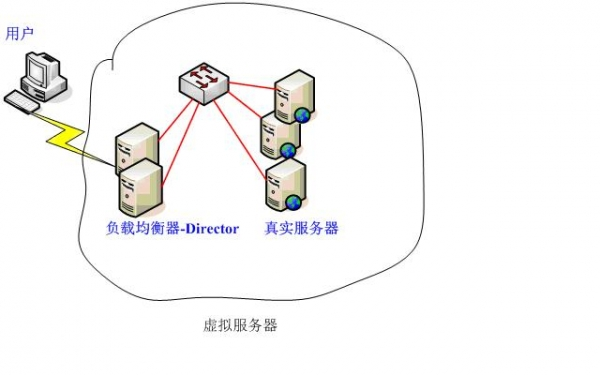
\includegraphics[keepaspectratio,width=0.5\paperwidth]{Pictures/Network/VirtualServer.jpg}
	\caption{虚拟服务器}
	\label{fig:VirtualServer}
	\end{center}
\end{figure}

虚拟服务器是负载均衡体系的基本架构,它分两层结构:转发器(Director)和真实服务器。图\ref{fig:VirtualServer}为虚拟服务器的结构示意。

为什么称虚拟服务器?因为从用户的角度看来,似乎只是一个服务器在提供服务。虚拟服务器最主要的功能是提供包转发和负载均衡,这个功能可以通过撰写ipvsadm脚本具体实现。虚拟服务器项目由章文嵩博士所贡献,目前已被添加到各种Linux发行版的内核。

故障隔离指虚拟服务器中的某个真实服务器(或某几个真实服务器)失效或发生故障,系统将自动把失效的服务器从转发队列中清理出去,从而保证用户访问的正确性;另一方面,当实效的服务器被修复以后,系统再自动地把它加入转发队列。

失败切换,这是针对负载均衡器Director采取的措施,在有两个负载均衡器Director的应用场景,当主负载均衡器(MASTER)失效或出现故障,备份负载均衡器(BACKUP)将自动接管主负载均衡器的工作;一旦主负载均衡器故障修复,两者将恢复到最初的角色。

要从技术上实现虚拟服务器、故障隔离及失败切换3个功能,需要两个工具:ipvsadm和keepalived。当然也有heartbeat这样的工具可以实现同样的功能,但相对于keepalived,heartbeat的实现要复杂得多(如撰写ipvsadm脚本,部署ldirectord,编写资源文件等)。在采用keepalived的方案里,只要ipvsadm被正确的安装,简单的配置唯一的文件keepalived就行了。


\subsection{LVS}
LVS是Linux Virtual Server的简写,意即Linux虚拟服务器,是一个虚拟的服务器集群系统。本项目在1998年5月由章文嵩博士成立,是中国国内最早出现的自由软件项目之一。

\begin{figure}[ht]
	\begin{center}
		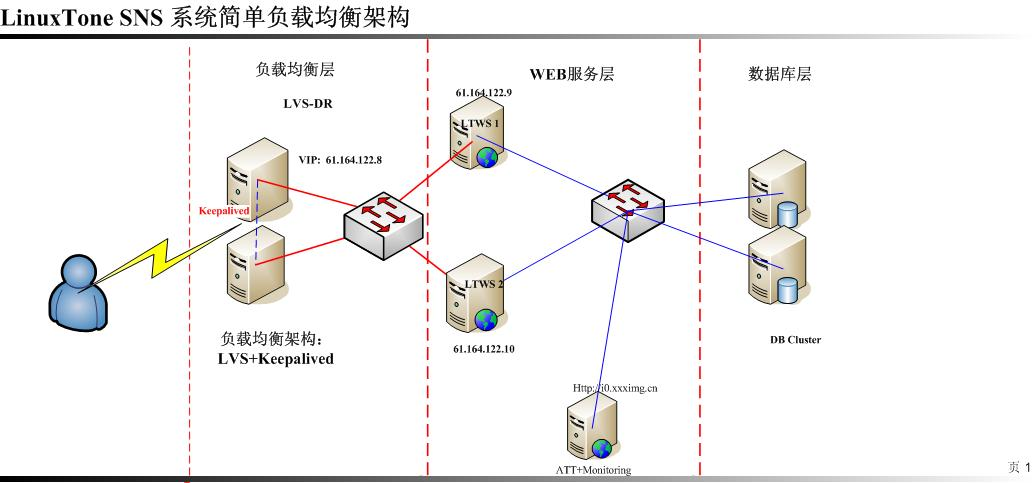
\includegraphics[keepaspectratio,width=0.5\paperwidth]{Pictures/Network/LinuxToneSnsArch.jpg}
	\caption{LinuxTone网站架构}
	\label{fig:LinuxToneSnsArch}
	\end{center}
\end{figure}

LVS常常与keepalived进行协作,如图\ref{fig:LinuxToneSnsArch}所示。


LVS集群采用IP负载均衡技术和基于内容请求分发技术。调度器具有很好的吞吐率,将请求均衡地转移到不同的服务器上执行,且调度器自动屏蔽掉服务器的故障,从而将一组服务器构成一个高性能的、高可用的虚拟服务器。整个服务器集群的结构对客户是透明的,而且无需修改客户端和服务器端的程序。为此,在设计时需要考虑系统的透明性、可伸缩性、高可用性和易管理性。
目前有三种IP负载均衡技术\textbf{(VS/NAT、VS/TUN和VS/DR)}。

一般来说,LVS集群采用三层结构,其主要组成部分为:
\begin{description}
\item[负载调度器(load balancer)] 它是整个集群对外面的前端机,它可以采用IP负载均衡技术、基于内容请求分发技术或者两者相结合
\item[服务器池(server pool)] 是一组真正执行客户请求的服务器,执行的服务有WEB、MAIL、FTP和DNS等
\item[共享存储(shared storage)] 它为服务器池提供一个共享的存储区,这样很容易使得服务器池拥有相同的内容,提供相同的服务
\end{description}


\subsection{IPVS}
IPVS(IP Virtual Server)是运行在LVS下的提供负载平衡功能的一种技术。

IPVS基本上是一种高效的Layer-4交换机,它提供负载平衡的功能。当一个TCP连接的初始SYN报文到达时,IPVS就选择一台服务器,将报文转发给它。此后通过查发报文的IP和TCP报文头地址,保证此连接的后继报文被转发到相同的服务器。这样,IPVS无法检查到请求的内容再选择服务器,这就要求后端的服务器组是提供相同的服务,不管请求被送到哪一台服务器,返回结果都应该是一样的。但是在有一些应用中后端的服务器可能功能不一,有的是提供HTML文档的Web服务器,有的是提供图片的Web服务器,有的是提供CGI的Web服务器。这时,就需要基于内容请求分发 (Content-Based Request Distribution),同时基于内容请求分发可以提高后端服务器上访问的局部性。

LVS的IP负载平衡技术就是通过IPVS模块来实现的,IPVS是LVS集群系统的核心软件,它的主要作用是:安装在Director Server上,同时在Director Server上虚拟出一个IP地址,用户必须通过这个虚拟的IP地址访问服务。这个虚拟IP一般称为LVS的VIP,即Virtual IP。访问的请求首先经过VIP到达负载调度器,然后由负载调度器从Real Server列表中选取一个服务节点响应用户的请求。

\subsection{Keepalived}
keepalived是一款失效转发机制的软件, 它的作用是检测web服务器的状态,如果有一台web服务器死机,或工作出现故障,Keepalived将检测到,并将有故障的web服务器从系统中剔除,当web服务器工作正常后Keepalived自动将web服务器加入到服务器群中,这些工作全部自动完成,不需要人工干涉,需要人工做的只是修复故障的web服务器。

网络在设计的时候必须考虑到冗余容灾,包括线路冗余,设备冗余等,防止网络存在单点故障,那在路由器或三层交换机处实现冗余就显得尤为重要,在网络里面有个协议就是来做这事的,这个协议就是VRRP协议,Keepalived就是巧用VRRP协议来实现高可用性(HA)的。keepalived完全遵守VRRP协议,包括竞选机制等等。


\begin{figure}[ht]
	\begin{center}
		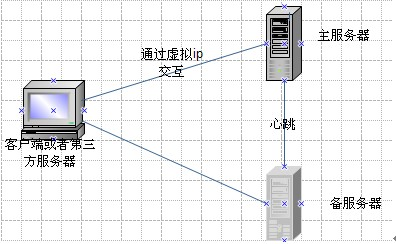
\includegraphics[keepaspectratio,width=0.5\paperwidth]{Pictures/Network/keepalivedIllus.jpg}
	\caption{Keepalived工作原理}
	\label{fig:keepalivedIllus}
	\end{center}
\end{figure}

图\ref{fig:keepalivedIllus}中主服务器和备服务器都装了keepalived软件,将keepalived配置成Master的便成了主服务器,将keepaliv-ed配置成BACKUP的自然就成了备服务器。主备服务器都通过keepalived绑定有相同的虚拟ip,外界就是利用这个虚拟ip与服务器进行交互的。正常情况下只有主服务器work,当主服务器宕机或者出现其他故障时Keepalived会将work转移到备服务器上,虚拟ip依然有效。当主服务器修复好了备用服务器会自动将work权利重新交给主服务器。 

keepalived也是模块化设计,不同模块复杂不同的功能,下面是keepalived的组件:

\begin{description}
\item[core]是keepalived的核心,复杂主进程的启动和维护,全局配置文件的加载解析等
\item[check]负责healthchecker(健康检查),包括了各种健康检查方式,以及对应的配置的解析包括LVS的配置解析
\item[vrrp]VRRPD子进程,VRRPD子进程就是来实现VRRP协议的
\item[libipfwc]iptables(ipchains)库,配置LVS会用到
\item[libipvs]配置LVS会用到
\end{description}

\begin{figure}[ht]
	\begin{center}
		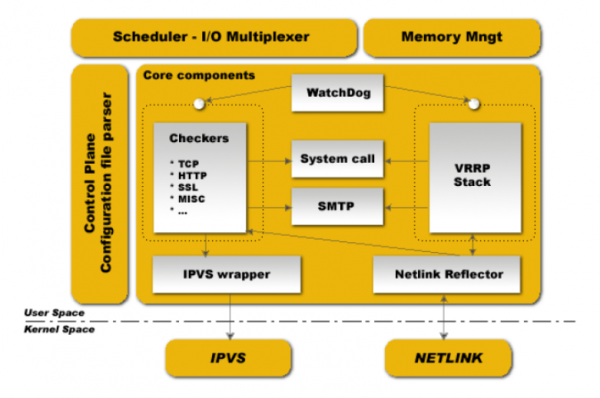
\includegraphics[keepaspectratio,width=0.5\paperwidth]{Pictures/Network/KeepalivedCore.png}
	\caption{Keepalived内部架构}
	\label{fig:KeepalivedCore}
	\end{center}
\end{figure}

keepalived启动后会有三个进程。父进程负责内存管理,子进程管理等等,两个子进程分别运行VRRP和healthchecker。
被系统WatchDog看管,healthchecker子进程复杂检查各自服务器的健康程度,例如HTTP,LVS等等,如果healthchecker子进程检查到MASTER上服务不可用了,就会通知本机上的兄弟VRRP子进程,让他删除通告,并且去掉虚拟IP,转换为BACKUP。

\subsection{Watchdog}

Carrier Grade Linux 是 OSDL(Open Source Development Lab)发布的电信级 Linux 的标准,在系统可用性这部分指出Linux必须支持 watchdog 机制。

Watchdog在实现上可以是硬件电路也可以是软件定时器,能够在系统出现故障时自动重新启动系统。在Linux 内核下, watchdog的基本工作原理是:当watchdog启动后(即/dev/watchdog 设备被打开后),如果在某一设定的时间间隔内/dev/watchdog没有被执行写操作, 硬件watchdog电路或软件定时器就会重新启动系统。

/dev/watchdog 是一个主设备号为10, 从设备号130的字符设备节点。 Linux内核不仅为各种不同类型的watchdog硬件电路提供了驱动,还提供了一个基于定时器的纯软件watchdog驱动。 驱动源码位于内核源码树drivers/char/watchdog/目录下。


\subsection{Memcached}

memcached是一套分布式的高速缓存系统,由LiveJournal的Brad Fitzpatrick开发,但目前被许多网站使用。这是一套开放源代码软件,以BSD license授权发布。

memcached缺乏认证以及安全管制,这代表应该将memcached服务器放置在防火墙后。

memcached的API使用三十二比特的循环冗余校验(CRC-32)计算键值后,将数据分散在不同的机器上。当表格满了以后,接下来新增的数据会以LRU机制替换掉。由于memcached通常只是当作高速缓存系统使用,所以使用memcached的应用程序在写回较慢的系统时(像是后端的数据库)需要额外的代码更新memcached内的数据。


\clearpage
%!Mode:: "TeX:UTF-8"
\section{并发架构}
我们在设计一个服务器的软件架构的时候,通常会考虑几种架构:
多进程(隔离性,在linux下面的服务程序广泛采用,比如大名鼎鼎的apache)、
多线程(这种模型在windows下面比较常见)、
非阻塞/异步IO(callback) 以及Coroutine模型。

网络服务在处理数以万计的客户端连接时,往往出现效率低下甚至完全瘫痪,这被称为C10K问题。

多进程和多线程都有资源耗费比较大的问题,所以在高并发量的服务器端使用并不多。
这里我们重点来研究一下两种架构,基于callback和coroutine的架构。




\subsection{Callback- 非阻塞/异步IO}
这种架构的特点是使用非阻塞的IO,这样服务器就可以持续运转,而不需要等待,可以使用很少的线程,即使只有一个也可以。需要定期的任务可以采取定时器来触发。把这种架构发挥到极致的就是node.js,一个用javascript来写服务器端程序的框架。在node.js中,所有的io都是non-block的,可以设置回调。

这种架构的缺点是编程复杂,把以前连续的流程切成了很多片段。另外也不能充分发挥多核的能力。
\subsection{Coroutine-协程}
coroutine本质上是一种轻量级的thread,它的开销会比使用thread少很多。多个coroutine可以按照次序在一个thread里面执行,一个coroutine如果处于block状态,可以交出执行权,让其他的coroutine继续执行。使用coroutine可以以清晰的编程模型实现状态机。

协程和一般多线程的区别是,一般多线程由系统决定该哪个线程执行,是抢占式的,而协程是由每个线程自己决定自己什么时候不执行,并把执行权主动交给下一个线程。 协程是用户空间线程,操作系统其存在一无所知,所以需要用户自己去做调度,用来执行协作式多任务非常合适。

线程和协同程序的主要不同在于:在多处理器情况下,多线程程序同时运行多个线程;而协同程序是通过协作来完成,在任一指定时刻只有一个协同程序在运行,并且这个正在运行的协同程序只在必要时才会被挂起。这样Lua的协程就不能利用现在多核技术了。

Lua 协程有三个状态:suspended,running,dead。可以通过coroutine.status来查看协程状态。


让我们看看Lua语言的coroutine的例子。
\begin{verbatim}
> function foo()
 >>   print("foo", 1)
 >>   coroutine.yield()
 >>   print("foo", 2)
 >> end
> co = coroutine.create(foo) -- create a coroutine with foo as the entry
> = coroutine.status(co)
 suspended
 > = coroutine.resume(co) <--第一次resume
 foo     1
 > = coroutine.resume(co) <--第二次resume
 foo     2
 > = coroutine.status(co)
 dead
\end{verbatim}
Google go语言也对coroutine使用了语言级别的支持,使用关键字go来启动一个coroutine(从这个关键字可以看出Go语言对coroutine的重视),结合chan(类似于message queue的概念)来实现coroutine的通讯,实现了Go的理念 ”Do not communicate by sharing memory; instead, share memory by communicating.”。一个例子:
\begin{verbatim}
func ComputeAValue(c chan float64) {
     // Do the computation.
     x := 2.3423 / 534.23423;
     c <- x;
 }
func UseAGoroutine() {
    channel := make(chan float64);
    go ComputeAValue(channel);
    // do something else for a while
    value := <- channel;
    fmt.Printf("Result was: %v", value);
 }
\end{verbatim}


在业务流程实现上,coroutine确实是更理想的实现,基于callback的风格,代码确实不是那么清晰。
但是现实世界中,coroutine到目前为止并没有真正流行起来,第一,是因为支持的语言并不是很多,比较新的语言(python/lua/go/erlang)才支持,但是老一些的语言(java/c/c++)并没有语言级别的支持。第二个原因是因为coroutine的使用可能让一些糟糕的代码占用过多的内存,而且比较难于排查。另外在实现一个工作流的构架中,流的暂停和恢复的时机都是未知的,系统的状态并不能放在内存中存放,都必须序列化,所以coroutine本身要提供序列化的机制,才可以实现稳定的系统。我想这些就是coroutine叫好不叫座的原因。

\subsection{Windows IOCP}
IOCP全称I/O Completion Port,中文译为I/O完成端口。IOCP是一个异步I/O的API,它可以高效地将I/O事件通知给应用程序。与使用select()或是其它异步方法不同的是,一个套接字[socket]与一个完成端口关联了起来,然后就可继续进行正常的Winsock操作了。然而,当一个事件发生的时候,此完成端口就将被操作系统加入一个队列中。然后应用程序可以对核心层进行查询以得到此完成端口。

\subsection{事件驱动的缺点}
不管是Nginx还是Squid这种反向代理,其网络模式都是事件驱动。事件驱动其实是很老的技术,早期的select、poll都是如此。后来基于内核通知的更高级事件机制出现,如libevent里的epoll,使事件驱动性能得以提高。事件驱动的本质还是IO事件,应用程序在多个IO句柄间快速切换,实现所谓的异步IO。事件驱动服务器,最适合做的就是这种IO密集型工作,如反向代理,它在客户端与WEB服务器之间起一个数据中转作用,纯粹是IO操作,自身并不涉及到复杂计算。

Apache或者Resin这类应用服务器,之所以称他们为应用服务器,是因为他们真的要跑具体的业务应用,如科学计算、图形图像、数据库读写等。它们很可能是CPU密集型的服务,事件驱动并不合适。例如一个计算耗时2秒,那么这2秒就是完全阻塞的,什么event都没用。想想MySQL如果改成事件驱动会怎么样,一个大型的join或sort就会阻塞住所有客户端。这个时候多进程或线程就体现出优势,每个进程各干各的事,互不阻塞和干扰。当然,现代CPU越来越快,单个计算阻塞的时间可能很小,但只要有阻塞,事件编程就毫无优势。所以进程、线程这类技术,并不会消失,而是与事件机制相辅相成,长期存在。

\subsection{多核系统}

Squid-3.3使用wokers 支持基本的多核,管理员可以通过配置启动一个squid来派生多个worker进程利用所有可利用的CPU。
Nginx也采用类似机制,通过多个worker进程绑定到CPU上。
























%!Mode:: "TeX:UTF-8"

\section{爬}




\hypersetup{colorlinks=true}
\href{http://www.crummy.com/software/BeautifulSoup/bs4/doc/}{beautifulsoup4官方文档}




























%!Mode:: "TeX:UTF-8"
\section{Curl工具}
 \begin{verbatim}
curl -svo /dev/null test/abc -x 127.0.0.1:2432

curl -X PUT \
     -H 'Content-Type: application/json' \
          -d '{"firstName":"Kris", "lastName":"Jordan"}'
               echo.httpkit.com

curl -X PUT \
     -H 'Content-Type: application/json' \
     -d @example.json
     echo.httpkit.com

curl -d "firstName=Kris" \
     -d "lastName=Jordan" \
     echo.httpkit.com

curl -F "firstName=Kris" \
     -F "publicKey=@idrsa.pub;type=text/plain" \
     echo.httpkit.com

 \end{verbatim}


-x 指定服务端地址

-H 指定头部值

-X 指定方法名

-A 指定User-Agent值

-o 指定本地保存文件名称

-O 使用同服务端相同的文件名称来保存

-d 指定请求body,以application/x-www-form-urlencoded类型发送,可用于发送JSON等消息体。使用@指定文件作为body

-F 指定HTML表格请求body,以multipart/form-data类型发送




%!Mode:: "TeX:UTF-8"
\section{GitHub Pages服务}

\begin{verbatim}
git push origin gitcafe-pages #GitCafe
git push origin master #GitHub
https://help.github.com/articles/using-jekyll-with-pages/
\end{verbatim}


安装jekyll的问题包括,官方源访问不稳定,mac自带的ruby太老。系统里有了两个版本的ruby后,各种不爽。


阮一峰关于Jekyll的简单介绍:
\url{http://www.ruanyifeng.com/blog/2012/08/blogging_with_jekyll.html}

安装rvm
\begin{verbatim}
curl -L get.rvm.io | bash -s stable
\end{verbatim}

其实,用jekyll只需一条命令就可以建站
\begin{verbatim}
jekyll new my-awesome-site
\end{verbatim}

Ruby Gem安装过程中会遇到问题,解决的诀窍,一是删除Gem.lock,二是bundle update,bundle install,三是更换到国内的淘宝源。

bundle clean --force


\url{http://taohui.org.cn/mywebbuild.html}


怎么解决云主机只有内网IP的问题?
将内网云主机的默认网关改到某台有外网的主机上。
%!Mode:: "TeX:UTF-8"
\section{Nginx}
Nginx(发音同engine x)是一款由俄罗斯程序员Igor Sysoev所开发轻量级的网页服务器、反向代理服务器以及电子邮件(IMAP/POP3)代理服务器。起初是供俄国大型的门户网站及搜索引擎Rambler使用。此软件BSD-like协议下发行,可以在UNIX、GNU/Linux、BSD、Mac OS X、Solaris,以及Microsoft Windows等操作系统中运行。

Nginx是一款面向性能设计的HTTP服务器,相较于Apache、lighttpd具有占有内存少,稳定性高等优势。与旧版本(<=2.2)的Apache不同,nginx不采用每客户机一线程的设计模型,而是充分使用异步逻辑,削减了上下文调度开销,所以并发服务能力更强。整体采用模块化设计,有丰富的模块库和第三方模块库,配置灵活。 在Linux操作系统下,nginx使用epoll事件模型,得益于此,nginx在Linux操作系统下效率相当高。同时Nginx在OpenBSD或FreeBSD操作系统上采用类似于epoll的高效事件模型kqueue。

\subsection{阶段}
Nginx将HTTP处理分为11个阶段(Phase):
\begin{description}
\item[PostRead]接收完请求头之后的第一个阶段,它位于uri重写之前,实际上很少有模块会注册在该阶段,默认的情况下,该阶段被跳过
\item[ServerRewrite]server级别的uri重写阶段,也就是该阶段执行处于server块内,location块外的重写指令
\item[FingConfig]重写URL后找到匹配的location块,其原理是从location组成的静态二叉树中快速检索。处理方法由官方提供不可更改。
\item[Rewrite]location级别的uri重写阶段,该阶段执行location基本的重写指令,也可能会被执行多次。同ServerRewrite完全相同,其checker函数也是\verb$ngx_http_core_rewrite_phase$。
\item[PostRewrite]location级别重写的后一阶段,用来检查上阶段是否有uri重写,并根据结果跳转到合适的阶段,并限制重写URL次数,防止死循环。处理方法由官方提供不可更改。
\item[PreAccess]访问权限控制的前一阶段,该阶段在权限控制阶段之前,一般也用于访问控制,比如限制访问频率,链接数等
\item[Access]访问权限控制阶段,比如基于ip黑白名单的权限控制,基于用户名密码的权限控制等
\item[PostAccess]访问权限控制的后一阶段,该阶段根据权限控制阶段的执行结果进行相应处理
\item[TryFiles]\verb$try_files$指令的处理阶段,如果没有配置\verb$try_files$指令,则该阶段被跳过。\verb$try_files$作用类似于rewrite,用于配置所请求内容的路径选择规则
\item[Content]内容生成阶段,该阶段产生响应,并发送到客户端
\item[Log]日志记录阶段,该阶段记录访问日志
\end{description}

在\verb$ngx_lua$中,有init, rewrite, access, set, content, log等阶段。

一般而言handler返回:
\begin{description}
\item [NGX\_OK]表示该阶段已经处理完成,需要转入下一个阶段
\item [NG\_DECLINED]表示需要转入本阶段的下一个handler继续处理
\item [NGX\_AGAIN, NGX\_DONE]表示需要等待某个事件发生才能继续处理(比如等待网络IO),此时Nginx为了不阻塞其他请求的处理,必须中断当前请求的执行链,等待事件发生之后继续执行该handler
\item [NGX\_ERROR]表示发生了错误,需要结束该请求
\end{description}



%!Mode:: "TeX:UTF-8"
\section{HTTP Range}
Range头域可以请求实体的一个或者多个子范围。例如,  
  表示头500个字节:bytes=0-499  
  表示第二个500字节:bytes=500-999  
  表示最后500个字节:bytes=-500  
  表示500字节以后的范围:bytes=500-  
  第一个和最后一个字节:bytes=0-0,-1  
  同时指定几个范围:bytes=500-600,601-999 

\section{HTTP状态码}

\subsection{1xx消息}
这一类型的状态码,代表请求已被接受,需要继续处理。这类响应是临时响应,只包含状态行和某些可选的响应头信息,并以空行结束。由于HTTP/1.0协议中没有定义任何1xx状态码,所以除非在某些试验条件下,服务器禁止向此类客户端发送1xx响应。 这些状态码代表的响应都是信息性的,标示客户应该采取的其他行动。

100 Continue
客户端应当继续发送请求。这个临时响应是用来通知客户端它的部分请求已经被服务器接收,且仍未被拒绝。客户端应当继续发送请求的剩余部分,或者如果请求已经完成,忽略这个响应。服务器必须在请求完成后向客户端发送一个最终响应。

101 Switching Protocols
服务器已经理解了客户端的请求,并将通过Upgrade消息头通知客户端采用不同的协议来完成这个请求。在发送完这个响应最后的空行后,服务器将会切换到在Upgrade消息头中定义的那些协议。
只有在切换新的协议更有好处的时候才应该采取类似措施。例如,切换到新的HTTP版本比旧版本更有优势,或者切换到一个实时且同步的协议以传送利用此类特性的资源。

102 Processing
由WebDAV(RFC 2518)扩展的状态码,代表处理将被继续执行。

\subsection{2xx成功}

这一类型的状态码,代表请求已成功被服务器接收、理解、并接受。

200 OK
请求已成功,请求所希望的响应头或数据体将随此响应返回。

201 Created
请求已经被实现,而且有一个新的资源已经依据请求的需要而创建,且其URI已经随Location头信息返回。假如需要的资源无法及时创建的话,应当返回'202 Accepted'。

202 Accepted
服务器已接受请求,但尚未处理。正如它可能被拒绝一样,最终该请求可能会也可能不会被执行。在异步操作的场合下,没有比发送这个状态码更方便的做法了。
返回202状态码的响应的目的是允许服务器接受其他过程的请求(例如某个每天只执行一次的基于批处理的操作),而不必让客户端一直保持与服务器的连接直到批处理操作全部完成。在接受请求处理并返回202状态码的响应应当在返回的实体中包含一些指示处理当前状态的信息,以及指向处理状态监视器或状态预测的指针,以便用户能够估计操作是否已经完成。

203 Non-Authoritative Information
服务器已成功处理了请求,但返回的实体头部元信息不是在原始服务器上有效的确定集合,而是来自本地或者第三方的拷贝。当前的信息可能是原始版本的子集或者超集。例如,包含资源的元数据可能导致原始服务器知道元信息的超集。使用此状态码不是必须的,而且只有在响应不使用此状态码便会返回200 OK的情况下才是合适的。

204 No Content
服务器成功处理了请求,但不需要返回任何实体内容,并且希望返回更新了的元信息。响应可能通过实体头部的形式,返回新的或更新后的元信息。如果存在这些头部信息,则应当与所请求的变量相呼应。
如果客户端是浏览器的话,那么用户浏览器应保留发送了该请求的页面,而不产生任何文档视图上的变化,即使按照规范新的或更新后的元信息应当被应用到用户浏览器活动视图中的文档。
由于204响应被禁止包含任何消息体,因此它始终以消息头后的第一个空行结尾。

205 Reset Content
服务器成功处理了请求,且没有返回任何内容。但是与204响应不同,返回此状态码的响应要求请求者重置文档视图。该响应主要是被用于接受用户输入后,立即重置表单,以便用户能够轻松地开始另一次输入。
与204响应一样,该响应也被禁止包含任何消息体,且以消息头后的第一个空行结束。

206 Partial Content
服务器已经成功处理了部分GET请求。类似于FlashGet或者迅雷这类的HTTP 下载工具都是使用此类响应实现断点续传或者将一个大文档分解为多个下载段同时下载。
该请求必须包含Range头信息来指示客户端希望得到的内容范围,并且可能包含If-Range来作为请求条件。
响应必须包含如下的头部域:

\begin{itemize}
\item Content-Range用以指示本次响应中返回的内容的范围;如果是Content-Type为multipart/byteranges的多段下载,则每一multipart段中都应包含Content-Range域用以指示本段的内容范围。假如响应中包含Content-Length,那么它的数值必须匹配它返回的内容范围的真实字节数。
\item Date
\item ETag和/或Content-Location,假如同样的请求本应该返回200响应。
\item Expires, Cache-Control,和/或Vary,假如其值可能与之前相同变量的其他响应对应的值不同的话。
\end{itemize}


假如本响应请求使用了If-Range强缓存验证,那么本次响应不应该包含其他实体头;假如本响应的请求使用了If-Range弱缓存验证,那么本次响应禁止包含其他实体头;这避免了缓存的实体内容和更新了的实体头信息之间的不一致。否则,本响应就应当包含所有本应该返回200响应中应当返回的所有实体头部域。
假如ETag或Last-Modified头部不能精确匹配的话,则客户端缓存应禁止将206响应返回的内容与之前任何缓存过的内容组合在一起。
任何不支持Range以及Content-Range头的缓存都禁止缓存206响应返回的内容。

207 Multi-Status
由WebDAV(RFC 2518)扩展的状态码,代表之后的消息体将是一个XML消息,并且可能依照之前子请求数量的不同,包含一系列独立的响应代码。

\subsection{3xx重定向}
这类状态码代表需要客户端采取进一步的操作才能完成请求。通常,这些状态码用来重定向,后续的请求地址(重定向目标)在本次响应的Location域中指明。

当且仅当后续的请求所使用的方法是GET或者HEAD时,用户浏览器才可以在没有用户介入的情况下自动提交所需要的后续请求。客户端应当自动监测无限循环重定向(例如:A→B→C→……→A或A→A),因为这会导致服务器和客户端大量不必要的资源消耗。按照HTTP/1.0版规范的建议,浏览器不应自动访问超过5次的重定向。

300 Multiple Choices
被请求的资源有一系列可供选择的回馈信息,每个都有自己特定的地址和浏览器驱动的商议信息。用户或浏览器能够自行选择一个首选的地址进行重定向。
除非这是一个HEAD请求,否则该响应应当包括一个资源特性及地址的列表的实体,以便用户或浏览器从中选择最合适的重定向地址。这个实体的格式由Content-Type定义的格式所决定。浏览器可能根据响应的格式以及浏览器自身能力,自动作出最合适的选择。当然,RFC 2616规范并没有规定这样的自动选择该如何进行。
如果服务器本身已经有了首选的回馈选择,那么在Location中应当指明这个回馈的URI;浏览器可能会将这个Location值作为自动重定向的地址。此外,除非额外指定,否则这个响应也是可缓存的。

301 Moved Permanently
被请求的资源已永久移动到新位置,并且将来任何对此资源的引用都应该使用本响应返回的若干个URI之一。如果可能,拥有链接编辑功能的客户端应当自动把请求的地址修改为从服务器反馈回来的地址。除非额外指定,否则这个响应也是可缓存的。
新的永久性的URI应当在响应的Location域中返回。除非这是一个HEAD请求,否则响应的实体中应当包含指向新的URI的超链接及简短说明。
如果这不是一个GET或者HEAD请求,因此浏览器禁止自动进行重定向,除非得到用户的确认,因为请求的条件可能因此发生变化。
注意:对于某些使用HTTP/1.0协议的浏览器,当它们发送的POST请求得到了一个301响应的话,接下来的重定向请求将会变成GET方式。

302 Found
请求的资源现在临时从不同的URI响应请求。由于这样的重定向是临时的,客户端应当继续向原有地址发送以后的请求。只有在Cache-Control或Expires中进行了指定的情况下,这个响应才是可缓存的。
新的临时性的URI应当在响应的Location域中返回。除非这是一个HEAD请求,否则响应的实体中应当包含指向新的URI的超链接及简短说明。
如果这不是一个GET或者HEAD请求,那么浏览器禁止自动进行重定向,除非得到用户的确认,因为请求的条件可能因此发生变化。
注意:虽然RFC 1945和RFC 2068规范不允许客户端在重定向时改变请求的方法,但是很多现存的浏览器将302响应视作为303响应,并且使用GET方式访问在Location中规定的URI,而无视原先请求的方法。状态码303和307被添加了进来,用以明确服务器期待客户端进行何种反应。

303 See Other
对应当前请求的响应可以在另一个URI上被找到,而且客户端应当采用GET的方式访问那个资源。这个方法的存在主要是为了允许由脚本激活的POST请求输出重定向到一个新的资源。这个新的URI不是原始资源的替代引用。同时,303响应禁止被缓存。当然,第二个请求(重定向)可能被缓存。
新的URI应当在响应的Location域中返回。除非这是一个HEAD请求,否则响应的实体中应当包含指向新的URI的超链接及简短说明。
注意:许多HTTP/1.1版以前的浏览器不能正确理解303状态。如果需要考虑与这些浏览器之间的互动,302状态码应该可以胜任,因为大多数的浏览器处理302响应时的方式恰恰就是上述规范要求客户端处理303响应时应当做的。

304 Not Modified
如果客户端发送了一个带条件的GET请求且该请求已被允许,而文档的内容(自上次访问以来或者根据请求的条件)并没有改变,则服务器应当返回这个状态码。304响应禁止包含消息体,因此始终以消息头后的第一个空行结尾。
该响应必须包含以下的头信息:
Date,除非这个服务器没有时钟。假如没有时钟的服务器也遵守这些规则,那么代理服务器以及客户端可以自行将Date字段添加到接收到的响应头中去(正如RFC 2068中规定的一样),缓存机制将会正常工作。
ETag和/或Content-Location,假如同样的请求本应返回200响应。
Expires, Cache-Control,和/或Vary,假如其值可能与之前相同变量的其他响应对应的值不同的话。
假如本响应请求使用了强缓存验证,那么本次响应不应该包含其他实体头;否则(例如,某个带条件的GET请求使用了弱缓存验证),本次响应禁止包含其他实体头;这避免了缓存了的实体内容和更新了的实体头信息之间的不一致。
假如某个304响应指明了当前某个实体没有缓存,那么缓存系统必须忽视这个响应,并且重复发送不包含限制条件的请求。
假如接收到一个要求更新某个缓存条目的304响应,那么缓存系统必须更新整个条目以反映所有在响应中被更新的字段的值。

305 Use Proxy
被请求的资源必须通过指定的代理才能被访问。Location域中将给出指定的代理所在的URI信息,接收者需要重复发送一个单独的请求,通过这个代理才能访问相应资源。只有原始服务器才能创建305响应。
注意:RFC 2068中没有明确305响应是为了重定向一个单独的请求,而且只能被原始服务器创建。忽视这些限制可能导致严重的安全后果。

306 Switch Proxy
在最新版的规范中,306状态码已经不再被使用。

307 Temporary Redirect
请求的资源现在临时从不同的URI响应请求。由于这样的重定向是临时的,客户端应当继续向原有地址发送以后的请求。只有在Cache-Control或Expires中进行了指定的情况下,这个响应才是可缓存的。
新的临时性的URI应当在响应的Location域中返回。除非这是一个HEAD请求,否则响应的实体中应当包含指向新的URI的超链接及简短说明。因为部分浏览器不能识别307响应,因此需要添加上述必要信息以便用户能够理解并向新的URI发出访问请求。
如果这不是一个GET或者HEAD请求,那么浏览器禁止自动进行重定向,除非得到用户的确认,因为请求的条件可能因此发生变化。

\subsection{4xx客户端错误}

这类的状态码代表了客户端看起来可能发生了错误,妨碍了服务器的处理。除非响应的是一个HEAD请求,否则服务器就应该返回一个解释当前错误状况的实体,以及这是临时的还是永久性的状况。这些状态码适用于任何请求方法。浏览器应当向用户显示任何包含在此类错误响应中的实体内容。

如果错误发生时客户端正在传送数据,那么使用TCP的服务器实现应当仔细确保在关闭客户端与服务器之间的连接之前,客户端已经收到了包含错误信息的数据包。如果客户端在收到错误信息后继续向服务器发送数据,服务器的TCP栈将向客户端发送一个重置数据包,以清除该客户端所有还未识别的输入缓冲,以免这些数据被服务器上的应用程序读取并干扰后者。

400 Bad Request
由于包含语法错误,当前请求无法被服务器理解。除非进行修改,否则客户端不应该重复提交这个请求。

401 Unauthorized
当前请求需要用户验证。该响应必须包含一个适用于被请求资源的WWW-Authenticate信息头用以询问用户信息。客户端可以重复提交一个包含恰当的Authorization头信息的请求。如果当前请求已经包含了Authorization证书,那么401响应代表着服务器验证已经拒绝了那些证书。如果401响应包含了与前一个响应相同的身份验证询问,且浏览器已经至少尝试了一次验证,那么浏览器应当向用户展示响应中包含的实体信息,因为这个实体信息中可能包含了相关诊断信息。参见RFC 2617。

402 Payment Required
该状态码是为了将来可能的需求而预留的。

403 Forbidden
服务器已经理解请求,但是拒绝执行它。与401响应不同的是,身份验证并不能提供任何帮助,而且这个请求也不应该被重复提交。如果这不是一个HEAD请求,而且服务器希望能够讲清楚为何请求不能被执行,那么就应该在实体内描述拒绝的原因。当然服务器也可以返回一个404响应,假如它不希望让客户端获得任何信息。

404 Not Found
请求失败,请求所希望得到的资源未被在服务器上发现。没有信息能够告诉用户这个状况到底是暂时的还是永久的。假如服务器知道情况的话,应当使用410状态码来告知旧资源因为某些内部的配置机制问题,已经永久的不可用,而且没有任何可以跳转的地址。404这个状态码被广泛应用于当服务器不想揭示到底为何请求被拒绝或者没有其他适合的响应可用的情况下。

405 Method Not Allowed
请求行中指定的请求方法不能被用于请求相应的资源。该响应必须返回一个Allow头信息用以表示出当前资源能够接受的请求方法的列表。
鉴于PUT,DELETE方法会对服务器上的资源进行写操作,因而绝大部分的网页服务器都不支持或者在默认配置下不允许上述请求方法,对于此类请求均会返回405错误。

406 Not Acceptable
请求的资源的内容特性无法满足请求头中的条件,因而无法生成响应实体。
除非这是一个HEAD请求,否则该响应就应当返回一个包含可以让用户或者浏览器从中选择最合适的实体特性以及地址列表的实体。实体的格式由Content-Type头中定义的媒体类型决定。浏览器可以根据格式及自身能力自行作出最佳选择。但是,规范中并没有定义任何作出此类自动选择的标准。

407 Proxy Authentication Required
与401响应类似,只不过客户端必须在代理服务器上进行身份验证。代理服务器必须返回一个Proxy-Authenticate用以进行身份询问。客户端可以返回一个Proxy-Authorization信息头用以验证。参见RFC 2617。

408 Request Timeout
请求超时。客户端没有在服务器预备等待的时间内完成一个请求的发送。客户端可以随时再次提交这一请求而无需进行任何更改。

409 Conflict
由于和被请求的资源的当前状态之间存在冲突,请求无法完成。这个代码只允许用在这样的情况下才能被使用:用户被认为能够解决冲突,并且会重新提交新的请求。该响应应当包含足够的信息以便用户发现冲突的源头。
冲突通常发生于对PUT请求的处理中。例如,在采用版本检查的环境下,某次PUT提交的对特定资源的修改请求所附带的版本信息与之前的某个(第三方)请求向冲突,那么此时服务器就应该返回一个409错误,告知用户请求无法完成。此时,响应实体中很可能会包含两个冲突版本之间的差异比较,以便用户重新提交归并以后的新版本。

410 Gone
被请求的资源在服务器上已经不再可用,而且没有任何已知的转发地址。这样的状况应当被认为是永久性的。如果可能,拥有链接编辑功能的客户端应当在获得用户许可后删除所有指向这个地址的引用。如果服务器不知道或者无法确定这个状况是否是永久的,那么就应该使用404状态码。除非额外说明,否则这个响应是可缓存的。
410响应的目的主要是帮助网站管理员维护网站,通知用户该资源已经不再可用,并且服务器拥有者希望所有指向这个资源的远端连接也被删除。这类事件在限时、增值服务中很普遍。同样,410响应也被用于通知客户端在当前服务器站点上,原本属于某个个人的资源已经不再可用。当然,是否需要把所有永久不可用的资源标记为'410 Gone',以及是否需要保持此标记多长时间,完全取决于服务器拥有者。

411 Length Required
服务器拒绝在没有定义Content-Length头的情况下接受请求。在添加了表明请求消息体长度的有效Content-Length头之后,客户端可以再次提交该请求。

412 Precondition Failed
服务器在验证在请求的头字段中给出先决条件时,没能满足其中的一个或多个。这个状态码允许客户端在获取资源时在请求的元信息(请求头字段数据)中设置先决条件,以此避免该请求方法被应用到其希望的内容以外的资源上。

413 Request Entity Too Large
服务器拒绝处理当前请求,因为该请求提交的实体数据大小超过了服务器愿意或者能够处理的范围。此种情况下,服务器可以关闭连接以免客户端继续发送此请求。
如果这个状况是临时的,服务器应当返回一个Retry-After的响应头,以告知客户端可以在多少时间以后重新尝试。

414 Request-URI Too Long
请求的URI长度超过了服务器能够解释的长度,因此服务器拒绝对该请求提供服务。这比较少见,通常的情况包括:
本应使用POST方法的表单提交变成了GET方法,导致查询字符串(Query String)过长。
重定向URI“黑洞”,例如每次重定向把旧的URI作为新的URI的一部分,导致在若干次重定向后URI超长。
客户端正在尝试利用某些服务器中存在的安全漏洞攻击服务器。这类服务器使用固定长度的缓冲读取或操作请求的URI,当GET后的参数超过某个数值后,可能会产生缓冲区溢出,导致任意代码被执行。没有此类漏洞的服务器,应当返回414状态码。

415 Unsupported Media Type
对于当前请求的方法和所请求的资源,请求中提交的实体并不是服务器中所支持的格式,因此请求被拒绝。

416 Requested Range Not Satisfiable
如果请求中包含了Range请求头,并且Range中指定的任何数据范围都与当前资源的可用范围不重合,同时请求中又没有定义If-Range请求头,那么服务器就应当返回416状态码。
假如Range使用的是字节范围,那么这种情况就是指请求指定的所有数据范围的首字节位置都超过了当前资源的长度。服务器也应当在返回416状态码的同时,包含一个Content-Range实体头,用以指明当前资源的长度。这个响应也被禁止使用multipart/byteranges作为其Content-Type。

417 Expectation Failed
在请求头Expect中指定的预期内容无法被服务器满足,或者这个服务器是一个代理服务器,它有明显的证据证明在当前路由的下一个节点上,Expect的内容无法被满足。

418 I'm a teapot
本操作码是在1998年作为IETF的传统愚人节笑话, 在RFC 2324 超文本咖啡壶控制协议中定义的,并不需要在真实的HTTP服务器中定义。

421 There are too many connections from your internet address
从当前客户端所在的IP地址到服务器的连接数超过了服务器许可的最大范围。通常,这里的IP地址指的是从服务器上看到的客户端地址(比如用户的网关或者代理服务器地址)。在这种情况下,连接数的计算可能涉及到不止一个终端用户。

422 Unprocessable Entity
请求格式正确,但是由于含有语义错误,无法响应。(RFC 4918 WebDAV)

423 Locked
当前资源被锁定。(RFC 4918 WebDAV)

424 Failed Dependency
由于之前的某个请求发生的错误,导致当前请求失败,例如PROPPATCH。(RFC 4918 WebDAV)

425 Unordered Collection
在WebDav Advanced Collections草案中定义,但是未出现在《WebDAV顺序集协议》(RFC 3658)中。

426 Upgrade Required
客户端应当切换到TLS/1.0。(RFC 2817)

449 Retry With
由微软扩展,代表请求应当在执行完适当的操作后进行重试。

\subsection{5xx服务器错误}
这类状态码代表了服务器在处理请求的过程中有错误或者异常状态发生,也有可能是服务器意识到以当前的软硬件资源无法完成对请求的处理。除非这是一个HEAD请求,否则服务器应当包含一个解释当前错误状态以及这个状况是临时的还是永久的解释信息实体。浏览器应当向用户展示任何在当前响应中被包含的实体。

这些状态码适用于任何响应方法。

500 Internal Server Error
服务器遇到了一个未曾预料的状况,导致了它无法完成对请求的处理。一般来说,这个问题都会在服务器的程序码出错时出现。

501 Not Implemented
服务器不支持当前请求所需要的某个功能。当服务器无法识别请求的方法,并且无法支持其对任何资源的请求。

502 Bad Gateway
作为网关或者代理工作的服务器尝试执行请求时,从上游服务器接收到无效的响应。

503 Service Unavailable
由于临时的服务器维护或者过载,服务器当前无法处理请求。这个状况是临时的,并且将在一段时间以后恢复。如果能够预计延迟时间,那么响应中可以包含一个Retry-After头用以标明这个延迟时间。如果没有给出这个Retry-After信息,那么客户端应当以处理500响应的方式处理它。

504 Gateway Timeout
作为网关或者代理工作的服务器尝试执行请求时,未能及时从上游服务器(URI标识出的服务器,例如HTTP、FTP、LDAP)或者辅助服务器(例如DNS)收到响应。
注意:某些代理服务器在DNS查询超时时会返回400或者500错误。

505 HTTP Version Not Supported
服务器不支持,或者拒绝支持在请求中使用的HTTP版本。这暗示着服务器不能或不愿使用与客户端相同的版本。响应中应当包含一个描述了为何版本不被支持以及服务器支持哪些协议的实体。

506 Variant Also Negotiates
由《透明内容协商协议》(RFC 2295)扩展,代表服务器存在内部配置错误:被请求的协商变元资源被配置为在透明内容协商中使用自己,因此在一个协商处理中不是一个合适的重点。

507 Insufficient Storage
服务器无法存储完成请求所必须的内容。这个状况被认为是临时的。(WebDAV RFC 4918)

509 Bandwidth Limit Exceeded
服务器达到带宽限制。这不是一个官方的状态码,但是仍被广泛使用。

510 Not Extended
获取资源所需要的策略并没有被满足。(RFC 2774)

 
 
 
 
 
 

%!Mode:: "TeX:UTF-8"
\section{代理服务器}

\subsection{反向代理}
反向代理(Reverse Proxy)方式是指以代理服务器来接受internet上的连接请求,然后将请求转发给内部网络上的服务器,并将从服务器上得到的结果返回给internet上请求连接的客户端,此时代理服务器对外就表现为一个服务器。

安全反向代理有许多用途:
可以提供从防火墙外部代理服务器到防火墙内部安全内容服务器的加密连接;
可以允许客户机安全地连接到代理服务器,从而有利于安全地传输信息(如信用卡号)。


正向、反向代理区别:
\begin{description}
\item[用途]正向代理的典型用途是为在防火墙内的局域网客户端提供访问Internet的途径。正向代理还可以使用缓冲特性减少网络使用率。反向代理的典型用途是将防火墙后面的服务器提供给Internet用户访问。反向代理还可以为后端的多台服务器提供负载平衡,或为后端较慢的服务器提供缓冲服务。另外,反向代理还可以启用高级URL策略和管理技术,从而使处于不同web服务器系统的web页面同时存在于同一个URL空间下。
\item[安全性]正向代理允许客户端通过它访问任意网站并且隐藏客户端自身,因此你必须采取安全措施以确保仅为经过授权的客户端提供服务。
反向代理对外都是透明的,访问者并不知道自己访问的是一个代理。
\end{description}

\subsection{翻墙}
长城防火墙(The Great Firewall)屏蔽网站有以下几种方式:
\begin{enumerate}
\item DNS污染
\item 特定IP地址屏蔽
\item TCP连接重置 
\item 间歇性完全封锁
\end{enumerate}

用户和代理服务器之间建立VPN来传输加密数据,数据又通过代理转发给目的服务器,从而实现翻墙访问。


\subsection{匿名}

代理服务器根据匿名程度区分:
\begin{description}
\item[高度匿名代理]高度匿名代理会将我们的数据包原封不动的转发,在服务端看来就好像真的是一个普通客户端在访问,而记录的IP是代理服务器的IP。
\item[普通匿名代理]普通匿名代理会在数据包上做一些改动,服务端上有可能发现这是个代理服务器,也有一定几率追查到你的真实IP。
代理服务器通常会加入的HTTP头有HTTP\_VIA和HTTP\_X\_FORWARDED\_FOR。
\item[透明代理]透明代理不但改动了我们的数据包,还会告诉服务器你的真实IP。这种代理除了能用缓存技术帮你提高浏览速度,能用内容过滤提高你的安全性之外,并无其他显著作用。(最常见的例子是:内网中的硬件防火墙)。透明代理的意思是客户端根本不需要知道有代理服务器的存在,它改编你的request fields(报文),并会传送真实IP,多用于路由器的NAT转发中。注意,加密的透明代理则是属于匿名代理,意思是不用设置使用代理了,例如Garden 2程序。
\item[间谍代理]间谍代理指组织或个人创建的,用于记录使用者传输的数据,然后进行研究、监控等目的代理服务器。
\end{description}

















%!Mode:: "TeX:UTF-8"
\section{Resin}
Resin是CAUCHO公司的产品,是一个非常流行的application server,对servlet和JSP提供了良好的支持,性能也比较优良,resin自身采用JAVA语言开发。

Resin是CAUCHO公司的产品,是一个非常流行的支持servlets和jsp的引擎,速度非常快。Resin本身包含了一个支持HTTP/1.1的WEB服务器。虽然它可以显示动态内容,但是它显示静态内容的能力也非常强,速度直逼APACHESERVER。许多站点都是使用该WEB服务器构建的。

Resin也可以和许多其他的WEB服务器一起工作,比如Apache server和IIS等。Resin支持Servlets 2.3标准和JSP 1.2标准。熟悉ASP和PHP的用户可以发现用Resin来进行JSP编程是件很容易的事情。

Resin支持负载平衡(Load balancing),可以增加WEB站点的可靠性。方法是增加服务器的数量。比如一台SERVER的错误率是1\%的话,那么支持负载平衡的两个Resin服务器就可以使错误率降到0.01\%。





%!Mode:: "TeX:UTF-8"

\section{Squid}

Squid Cache(简称为Squid)是HTTP代理服务器软件。Squid用途广泛的,可以作为缓存服务器,可以过滤流量帮助网络安全,也可以作为代理服务器链中的一环,向上级代理转发数据或直接连接互联网。Squid程序在Unix一类系统运行。由于它是开源软件,有网站修改Squid的源代码,编译为原生Windows版;用户也可在Windows里安装Cygwin,然后在Cygwin里编译Squid。
\begin{figure}[ht]
	\begin{center}
		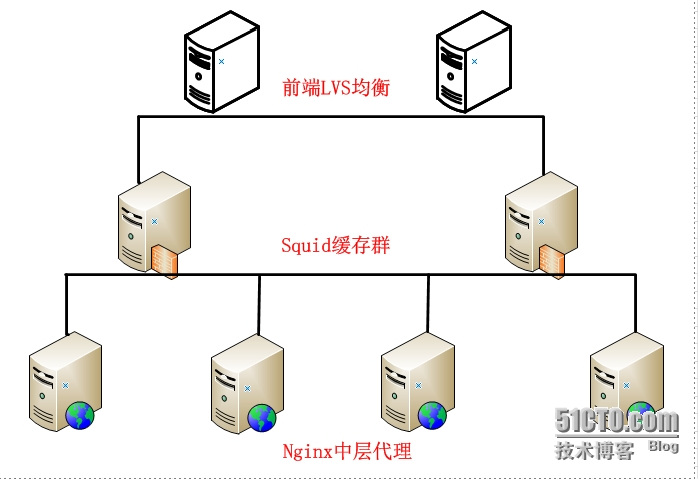
\includegraphics[keepaspectratio,width=0.3\paperwidth]{Pictures/Network/LvsPlusSquidPlusNginx.jpg}
		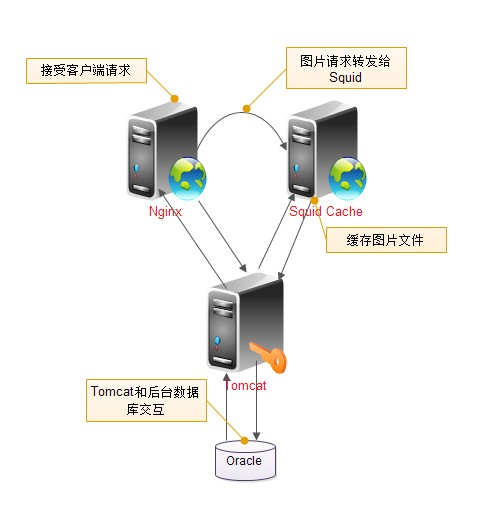
\includegraphics[keepaspectratio,width=0.3\paperwidth]{Pictures/Network/Nginx2Squid2Tomcat.jpg}
	\caption{Squid用作缓存服务器}
	\label{fig:LvsPlusSquidPlusNginx}
	\end{center}
\end{figure}


Squid的发展历史相当悠久,功能也相当完善。除了HTTP外,对于FTP与HTTPS的支持也相当好,在3.0测试版中也支持了IPv6。但是Squid的上级代理不能使用SOCKS协议。




\clearpage




%!Mode:: "TeX:UTF-8"
\section{流媒体防盗链技术}

《CDN技术详解》一书6.4.6节列举出了7种流媒体防盗链技术:

\begin{enumerate}
\item HTTP Referer检查
\item 验证登陆信息。登陆Session ID在Cookie中,也可将该登陆信息提取出来植入URL。这个方法不适合免登陆观看的视频内容。注意防盗链不是限制用户的获取,而是限制用户在其他网站获取。
\item Cookie中预先存入验证信息,比如一个字符串或数字
\item 使用Post方法下载。将下载链接换成一个表单和一个按钮,用户点击按钮。服务器验证是否是Post方法。\textit{我的理解是,点击URL后返回的是一个表单。盗链网站没法对表单进行手动处理。}
\item 使用图形验证码。\textit{我的理解是,同上一条类似,盗链系统无法做到让用户进行手动操作}。
\item 使用动态密钥。点击资源后,服务器计算一个临时的key,植入URL。用户再利用该URL进行访问。\textit{那么这个URL怎么返回给用户?通过302?盗链网站处理不了302?亦或是初次点击网址时返回的是Javascript代码?}
\item 在内容中插入随机字节。比如mp3的tag区,rar、zip的备注区,这样整个文件的哈希值会改变。其实是上一条方法的特例,即URL植入的临时key是哈希值。这个key既能用于合法性校验,又能进行哈希校验。\textit{服务器为什么要执行哈希校验?这不是客户端干的事情吗?}
\end{enumerate}


蓝汛HPCC实现了通用时间戳防盗链模块,我的理解是,URL中的时间戳那段每隔一段时间就更新一次,盗链网站无法做到及时更新。
更改URL意味着同时改变前端显示的URL和服务器记录的URL。客户端看到的URL未必是写死在html中的,可能是根据时间算出来的,为动态URL。
合法网站能够动态计算URL,加入时间戳,而非法网站只是点击一个死的URL。同理,服务器也不存一个死的url,也只是验证用户发来的URL。

湖南卫视要求蓝汛实现的防盗链算法中,需要在URL中植入时间戳和一段key,这个key是对路径、时间戳和密钥的哈希。密钥是一段简单的字符串,几乎是英文。如何把密钥传给客户端?太不安全。可能需要在点播时另外再建立一个连接,将原始URL(其实就是告诉服务端我想看哪个视频)发给服务器,服务器在服务端算好密钥然后生成新的URL返回给客户端,客户端用新的URL而非原始URL进行访问。但湖南卫视并未让蓝汛计算这个key,只让他验证这个key,说明这个key是在客户端计算的。



搜狐的服务端防盗链算法中,要求如果发现包含某个非法字符串,就返回404。我猜测其中原理是写死的网址都是包含这个非法串的,但是如果是在合法的网页下点击,实际发出的URL会去掉这个非法串。


综上,防盗链主要用到三种思路:
\begin{enumerate}
\item 检查盗链网站的HTTP referer。据说网页播放器不会传递Referer,不能使用这个手段。
\item 检查盗链网站的Cookie。不适合开放的资源。
\item 假定盗链网站不支持某些操作,如输入图形验证码,点击表单页的按钮,redirect到新的URL(?),这些操作只有用户+浏览器可以执行。\textit{如果盗链网站硬是模仿浏览器行为,也没办法,只能在于减少而非杜绝盗链}
\item 动态网页生成动态URL。不属于《CDN技术详解》上的七条。\textit{动态URL的生成原理是使用了JS?}
\end{enumerate}



%!Mode:: "TeX:UTF-8"
\section{Varnish}
Varnish是一款高性能的开源HTTP加速器,挪威最大的在线报纸 Verdens Gang 使用3台Varnish代替了原来的12台Squid,性能比以前更好。
Varnish 的作者Poul-Henning Kamp是FreeBSD的内核开发者之一,他认为现在的计算机比起1975年已经复杂许多。在1975年时,储存媒介只有两种:内存与硬盘。但现在计算机系统的内存除了主存外,还包括了CPU内的L1、L2,甚至有L3快取。硬盘上也有自己的快取装置,因此Squid Cache自行处理物件替换的架构不可能得知这些情况而做到最佳化,但操作系统可以得知这些情况,所以这部份的工作应该交给操作系统处理,这就是 Varnish cache设计架构。

Varnish is an HTTP accelerator designed for content-heavy dynamic web sites. In contrast to other web accelerators, such as Squid, which began life as a client-side cache, or Apache and nginx, which are primarily origin servers, Varnish was designed as an HTTP accelerator. Varnish is focused exclusively on HTTP, unlike other proxy servers that often support FTP, SMTP and other network protocols.

Varnish stores data in virtual memory and leaves the task of deciding what is stored in memory and what gets paged out to disk to the operating system. This helps avoid the situation where the operating system starts caching data while it is moved to disk by the application.

Furthermore, Varnish is heavily threaded, with each client connection being handled by a separate worker thread. When the configured limit on the number of active worker threads is reached, incoming connections are placed in an overflow queue; when this queue reaches its configured limit incoming connections will be rejected.

The principal configuration mechanism is Varnish Configuration Language (VCL), a domain-specific language (DSL) used to write hooks that are called at critical points in the handling of each request. Most policy decisions are left to VCL code, making Varnish more configurable and adaptable than most other HTTP accelerators. When a VCL script is loaded, it is translated to C, compiled to a shared object by the system compiler, and loaded directly into the accelerator.

A number of run-time parameters control things such as the maximum and minimum number of worker threads, various timeouts, etc. A command-line management interface allows these parameters to be modified, and new VCL scripts to be compiled, loaded and activated, without restarting the accelerator.

In order to reduce the number of system calls in the fast path to a minimum, log data is stored in shared memory, and the task of filtering, formatting and writing log data to disk is delegated to a separate application.


Varnish是一个轻量级的Cache和反向代理软件,先进的设计理念和成熟的设计框架是Varnish的主要特点,现在的Varnish总共代码量不大,功能上虽然在不断改进,但是还需要继续丰富和加强。
下面总结了Varnish的一些特点:\\
 (1)是基于内存缓存,重启后数据将消失。\\
 (2)利用虚拟内存方式,io性能好。\\
 (3)支持设置0~60秒内的精确缓存时间。\\
 (4)VCL配置管理比较灵活。\\
 (5)32位机器上缓存文件大小为最大2G。\\
 (6)具有强大的管理功能,例如top,stat,admin,list等。\\
 (7)状态机设计巧妙,结构清晰。\\
 (8)利用二叉堆管理缓存文件,达到积极删除目的。\\
 

Squid是一个高性能的代理缓存服务器,它和varnish之间有诸多的异同点,这里分析如下:
 下面是他们之间的相同点:(1)都是一个反向代理服务器, (2)都是开源软件。
 
 下面是它们的不同点,也是Varnish的优点:\\
 (1)Varnish的稳定性很高,两者在完成相同负荷的工作时,Squid服务器发生故障的几率要高于Varnish,因为使用Squid要经常重启。\\
 (2)Varnish访问速度更快,Varnish采用了“Visual Page Cache”技术,所有缓存数据都直接从内存读取,而squid是从硬盘读取,因而Varnish在访问速度方面会更快。\\
 (3)Varnish可以支持更多的并发连接,因为Varnish的TCP连接释放要比Squid快。因而在高并发连接情况下可以支持更多TCP连接。\\
 (4)Varnish可以通过管理端口,使用正则表达式批量的清除部分缓存,而Squid是做不到的。\\
 当然,与传统的Squid相比,Varnish也是有缺点的,列举如下:\\
 (1)varnish在高并发状态下CPU、IO、内存等资源开销都高于Squid。\\
 (2)varnish进程一旦Hang、Crash或者重启,缓存数据都会从内存中完全释放,此时所有请求都会发送到后端服务器,在高并发情况下,会给后端服务器造成很大压力。\\



%!Mode:: "TeX:UTF-8"
\section{VRRP}
VRRP(Virtual Router Redundancy Protocol)协议是用于实现路由器冗余的协议,最新协议在RFC3768中定义,原来的定义RFC2338被废除,新协议相对还简化了一些功能。

VRRP协议是为消除在静态缺省路由环境下的缺省路由器单点故障引起的网络失效而设计的主备模式的协议,使得在发生故障而进行设备功能切换时可以不影响内外数据通信,不需要再修改内部网络的网络参数。VRRP协议需要具有IP地址备份,优先路由选择,减少不必要的路由器间通信等功能。

 VRRP协议将两台或多台路由器设备虚拟成一个设备,对外提供虚拟路由器IP(一个或多个),而在路由器组内部,如果实际拥有这个对外IP的路由器如果工作正常的话就是MASTER,或者是通过算法选举产生,MASTER实现针对虚拟路由器IP的各种网络功能,如ARP请求,ICMP,以及数据的转发等;其他设备不拥有该IP,状态是BACKUP,除了接收MASTER的VRRP状态通告信息外,不执行对外的网络功能。当主机失效时,BACKUP将接管原先MASTER的网络功能。

 配置VRRP协议时需要配置每个路由器的虚拟路由器ID(VRID)和优先权值,使用VRID将路由器进行分组,具有相同VRID值的路由器为同一个组,VRID是一个0~255的正整数;同一组中的路由器通过使用优先权值来选举MASTER,优先权大者为MASTER,优先权也是一个0~255的正整数。

 VRRP协议使用多播数据来传输VRRP数据,VRRP数据使用特殊的虚拟源MAC地址发送数据而不是自身网卡的MAC地址,VRRP运行时只有MASTER路由器定时发送VRRP通告信息,表示MASTER工作正常以及虚拟路由器IP(组),BACKUP只接收VRRP数据,不发送数据,如果一定时间内没有接收到MASTER的通告信息,各BACKUP将宣告自己成为MASTER,发送通告信息,重新进行MASTER选举状态。

MASTER选举过程:\\
如果对外的虚拟路由器IP就是路由器本身配置的IP地址的话,该路由器始终都是MASTER;
否则如果不具备虚拟IP的话,将进行MASTER选举,各路由器都宣告自己是MASTER,发送VRRP通告信息;
如果收到其他机器的发来的通告信息的优先级比自己高,将转回BACKUP状态;
如果优先级相等的话,将比较路由器的实际IP,IP值较大的优先权高;
不过如果对外的虚拟路由器IP就是路由器本身的IP的话,该路由器始终将是MASTER,这时的优先级值为255。

VRRP协议状态比较简单,就三种状态,初始化,主机,备份机。

\begin{verbatim}
                      +---------------+
           +--------->|               |<-------------+
           |          |  Initialize   |              |
           |   +------|               |----------+   |
           |   |      +---------------+          |   |
           |   |                                 |   |
           |   V                                 V   |
   +---------------+                       +---------------+
   |               |---------------------->|               |
   |    Master     |                       |    Backup     |
   |               |<----------------------|               |
   +---------------+                       +---------------+
\end{verbatim}
   
   \begin{description}
   \item[初始化]路由器启动时,如果路由器的优先级是255(最高优先级,路由器拥有路由器地址),要发送VRRP通告信息,并发送广播ARP信息通告路由器IP地址对应的MAC地址为路由虚拟MAC,设置通告信息定时器准备定时发送VRRP通告信息,转为MASTER状态;
否则进入BACKUP状态,设置定时器检查定时检查是否收到MASTER的通告信息。
\item[主(master)机]主机状态下的路由器要完成如下功能:
 设置定时通告定时器;
 用VRRP虚拟MAC地址响应路由器IP地址的ARP请求;
 转发目的MAC是VRRP虚拟MAC的数据包;
 如果是虚拟路由器IP的拥有者,将接受目的地址是虚拟路由器IP的数据包,否则丢弃;
 当收到shutdown的事件时删除定时通告定时器,发送优先权级为0的通告包,转初始化状态;
 如果定时通告定时器超时时,发送VRRP通告信息;
 收到VRRP通告信息时,如果优先权为0,发送VRRP通告信息;否则判断数据的优先级是否高于本机,或相等而且实际IP地址大于本地实际IP,设置定时通告定时器,复位主机超时定时器,转BACKUP状态;否则的话,丢弃该通告包;
\item[备机] 备机状态下的路由器要实现以下功能:
 设置主机超时定时器;
 不能响应针对虚拟路由器IP的ARP请求信息;
 丢弃所有目的MAC地址是虚拟路由器MAC地址的数据包;
 不接受目的是虚拟路由器IP的所有数据包;
 当收到shutdown的事件时删除主机超时定时器,转初始化状态;
 主机超时定时器超时的时候,发送VRRP通告信息,广播ARP地址信息,转MASTER状态;
 收到VRRP通告信息时,如果优先权为0,表示进入MASTER选举;否则判断数据的优先级是否高于本机,如果高的话承认MASTER有效,复位主机超时定时器;否则的话,丢弃该通告包;
\end{description}


当内部主机通过ARP查询虚拟路由器IP地址对应的MAC地址时,MASTER路由器回复的MAC地址为虚拟的VRRP的MAC地址,而不是实际网卡的MAC地址,这样在路由器切换时让内网机器觉察不到;而在路由器重新启动时,不能主动发送本机网卡的实际MAC地址。如果虚拟路由器开启的ARP代理(proxy\_arp)功能,代理的ARP回应也回应VRRP虚拟MAC地址。

VRRP应用举例:\\

\begin{verbatim}
            +-----------+      +-----------+
            |   Rtr1    |      |   Rtr2    |
            |(MR VRID=1)|      |(BR VRID=1)|
            |(BR VRID=2)|      |(MR VRID=2)|
    VRID=1  +-----------+      +-----------+  VRID=2
    IP A ---------->*            *<---------- IP B
                    |            |
                    |            |
  ------------------+------------+-----+--------+--------+--------+--
                                       ^        ^        ^        ^
                                       |        |        |        |
                                     (IP A)   (IP A)   (IP B)   (IP B)
                                       |        |        |        |
                                    +--+--+  +--+--+  +--+--+  +--+--+
                                    |  H1 |  |  H2 |  |  H3 |  |  H4 |
                                    +-----+  +-----+  +--+--+  +--+--+
     Legend:
              ---+---+---+--  =  Ethernet, Token Ring, or FDDI
                           H  =  Host computer
                          MR  =  Master Router
                          BR  =  Backup Router
                           *  =  IP Address
                        (IP)  =  default router for hosts
\end{verbatim}

这是通常VRRP使用拓扑,两台路由器运行VRRP互为备份,路由器1作为VRID组1的MASTER,IP地址A,VRID组2的BACKUP,路由器2作为VRID组2的MASTER,IP地址B,VRID组1的BACKUP,内部网络中一部分机器的缺省网关地址是IP地址A,一部分是IP地址B,正常情况下以A为网关的数据将走路由器1,以B为网关的数据将走路由器2,如果一台路由器发生故障,所有数据将走另一台路由器。












\section{Web开发技术}


Python Web开发框架主要有Django, tornado,web2py, web,py等。

Cinatra为高性能现代C++ Web框架。

\subsection{HTML5}
HTML5支持的视频格式包括:mp4,ogg,webm。支持音频格式Ogg vorbis,mp3,wav。

\subsection{开发平台}


Baas:
\begin{verbatim}
https://leancloud.cn/
\end{verbatim}

图床:
\begin{verbatim}
http://tuchuang.org/
http://yotuku.cn/
http://m.yea.im/
http://www.poco.cn/
http://photo.weibo.com/
\end{verbatim}


\subsection{Django}


\begin{verbatim}
pip install mysql-python
\end{verbatim}




%!Mode:: "TeX:UTF-8"
\section{Web前端知识}
HTML5支持的视频格式包括:mp4,ogg,webm。支持音频格式Ogg vorbis,mp3,wav。


%!Mode:: "TeX:UTF-8"
\section{wget下载网站}
例如:
\begin{lstlisting}
wget -r -p -np -k http://www.21cn.com
wget --ftp-user=... --ftp-password=PASS  -r -p -np -k ftp://www.21cn.com
wget -r -p -np -k http://192.168.1.199/svn/OCTEON-SDK/branches/2012-03-27/OCTEON-SDK/docs/ --user=limz --password=123456
\end{lstlisting}






\end{document}
